\begin{figure}[ht]
\begin{doublespacing}
	\begin{minipage}[b]{0.4\linewidth}
		\hspace{1cm}
		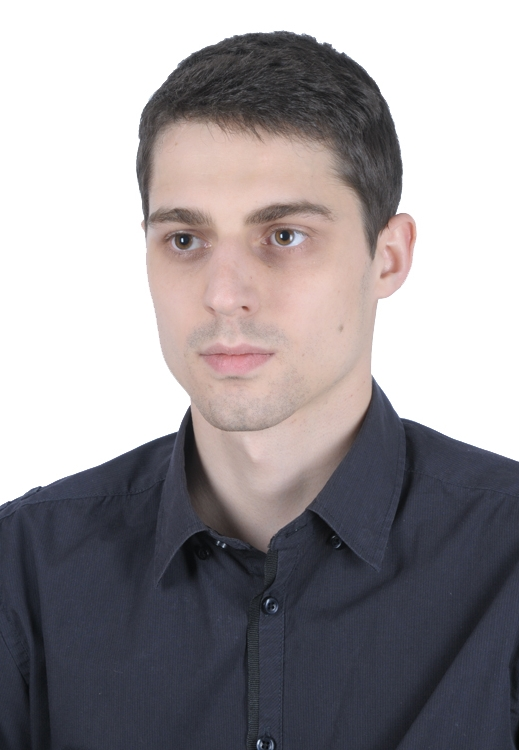
\includegraphics[width=4cm]{img/cv/me}
	\end{minipage}
	\begin{minipage}[b]{0.5\linewidth}
		Ireneusz Marek Szulc \\
		Kierunek:  Automatyka i Robotyka \\
		Specjalność:  Informatyka Przemysłowa \\
		Data urodzenia:  21.03.1993 r. \\
		Data rozpoczęcia studiów:  23.02.2016 r. \\
	\end{minipage}
	
	\hspace{2cm}
	
	\begin{center}
		\Large{\textbf{Życiorys}} \\
	\end{center}

Urodziłem się 21. marca 1993 roku w Lublinie. W 2012 roku rozpocząłem studia inżynierskie I stopnia na Wydziale Mechatroniki Politechniki Warszawskiej, na kierunku Automatyka i Robotyka, na specjalności Informatyka Przemysłowa. Ukończyłem je 17 lutego 2016 roku z wynikiem celującym. W tym samym roku rozpocząłem studia magisterskie na tym samym wydziale, na specjalności Informatyka Przemysłowa. \\

	\vspace{2cm}
	% podpis
	\begin{flushright}
				.............................................. \\
	\end{flushright}
\end{doublespacing}
\end{figure}


